
\chapter{Premesse}
\minitoc\mtcskip

\section{Introduzione}
L'uso in costante aumento di dispositivi mobili computerizzati spinge ogni sviluppatore a domandarsi
quali possano essere le loro applicazioni pratiche; conseguentemente
conoscendone  potenzialità e caratteristiche tecniche, si
chiede se gli stessi programmi che utilizza quotidianamente, possano essere
utilizzati senza la necessità - e la voglia - di reinventare la ruota.

Questo desiderio, spinto dalla necessità pratica, lo orienta a scegliere
sistemi di sviluppo che gli permettano di indagare le problematiche ed approfondirne
le soluzioni accreditate: per questo le ``piattaforme di sviluppo'' che si vanno via via
affermando - se non già consolidando - sono costituite dai sistemi operativi
GNU/Linux ed Android.

La seconda pone delle prosepettive interessanti, vuoi per l'utilizzo di una versione
del Kernel ottenuta dal \textit{fork} della prima, vuoi per il crescente interesse nel
mondo delle imprese, vuoi per le limitazioni architetturali imposte dagli stessi
sviluppatori. Queste ultime consentono agli hacker di sfruttare - vedi il rooting - 
le conoscenze sulle debolezze dei sistemi GNU/Linux allo scopo di superare
tali restrizioni, consentendo all'appassionato di conoscere meglio
il mondo GNU/Linux tramite l'analisi delle differenze architetturali
tra i due sistemi.
\bigskip

Entrando ora nel merito di questa Tesi di Laurea, il tentativo di \textit{porting}
di Pjproject - di per se già iniziato dalla comunità di sviluppatori, ma non
ancora portato a termine durante la redazione della presente - ha permesso di conoscere
sia l'oggetto iniziale di analisi, sia di scoprire nuovi aspetti sul \textit{porting}
e sulla piattaforma Android. Sebbene esistano tentativi di \textit{porting} basati 
sull'ideazione di Applicazioni Java o Applicazioni Native con JNI, lo scopo
perseguito è quello di utilizzare  il linguaggio 
C, allo scopo di interagire direttamente con il livelli architetturali il più
possibile vicini al Kernel e di distaccarsi dall'emulazione dei programmi tramite
la \textsc{Dalvik Virtual Machine}.

Questa tesi vorrà mostrare come questo tentativo non consenta l'evasione completa
dalla ``sandbox'' imposta da Google - benché questa si ottenga parzialmente
tramite tecniche di rooting - in quanto le librerie che vengono rese disponibili
all'interno dei dispositivi interagiscono direttamente con gli stati di controllo,
che limitano la configurabilità e l'utilizzo degli stessi.

Voglio inoltre mostrare quale sia l'architettura interna di tale sistema operativo,
senza tuttavia perdere di vista le difficoltà riscontrate nello svolgimento
del progetto, dovute sia all'immaturità del progetto Pjproject, sia sul mancato
testing dello stesso su alcuni aspetti, sia da mie considerazioni iniziali errate,
che sono state corrette durante il processo di analisi.

Questa sarà inoltre l'occasione per discorrere su quali strumenti utilizzare - ed 
in quale modo - allo scopo di ottenere i risultati che mostrerò via via.



\section{Terminologia adottata all'interno della tesi}
È necessario definire a priori una terminologia, onde chiarire alcune termini
ambigui. Per quanto riguarda le applicazioni, definisco:
\begin{description}
\item[Applicazioni Java] Questo genere di applicazioni sono quelle più diffuse
	all'interno del mondo Android: tutto il codice è scritto in linguaggio 
	Java, compreso l'accesso ai servizi di sistema, ed è necessario stabilire
	tramite Android Manifest file i permessi che si ritiene opportuno 
	utilizzare. Per la compilazione è sufficiente disporre dell'Android
	SDK.
\item[Applicazioni Native con JNI] In genere si fa riferimento a questo tipo di
	applicazioni come ad ``Applicazioni Native'' assieme alle successive
	\parencite[vedi][27-54]{libro:games} anche se, in questo caso, si
	accede alla Java Native Interface allo scopo di interagire con il codice Java. 
	La compilazione di queste applicazioni avviene tramite lo script 
	\texttt{\small ndk-build}, in ogni caso, viene sempre prodotto un file apk, 
	e vengono stabiliti i permessi di accesso nel Manifest. Per la compilazione 
	è necessario disporre dell'Android NDK.
\item[Applicazioni Native] Con questo termine faccio riferimento unicamente
	alle applicazioni compilate in codice binario, ed eseguibile direttamente
	dal processore. In genere si effettua la compilazione dei binari tramite
	Android NDK, ma è possibile utilizzare altri tool per il \textit{crosscompiling} preesistenti
	quali CodeSourcery Lite o la creazione di nuovi, in particolare tramite 
	crosstool-ng.
\end{description}
Si utilizzerà invece il termine generico di \textit{applicazione} qualora si faccia
riferimento indistintamente a tutte le tipologie di applicazione di cui sopra.

\begin{description}
\item[Kernel Android] Con questo termine si fa riferimento alla componente del	
	sistema operativo che comprende la versione modificata del Kernel Linux,
	facilmente ottenibile dal repository Git \url{https://android.googlesource.com/kernel/common}.
\item[AOSP Source] Con questo termine (acronimo di \textsc{Android Open Source Project}),
	si intende  la sovrastruttura costruita al 
	di sopra del Kernel Android. Questo sorgente tuttavia non include lo strato 
	del Kernel Android, come tra l'altro provato dalla Figura \vref{fig:androidsourceView}.
	
	Questi sorgenti mettono a disposizione le librerie di sistema per le
	applicazioni native in genere, le API per le applicazioni Java ed i 
	\textit{frameworks} (v. \ref{sec:explainframe}) per gestire lo stato del sistema: in genere con il termine
	\textbf{Android Middleware} \parencite{art:middleware} si fa riferimento all'insieme delle \textit{features}
	messe a disposizione dall'AOSP Source, e che forniscono alle applicazioni
	in esecuzione un'astrazione del sistema operativo.
\end{description}

Con il termine \textit{host} intendo il dispositivo sul quale si sta effettuando
il processo di cross-compilazione per la macchina di destinazione, detta
appunto \textit{target}.
\bigskip

Con il termine \textit{upsyscall} (o \textit{Up System Call}) mi riferirò alla possibilità
di richiamare, da strati di codice più elementari come quelli preposti dal codice
nativo ed in esecuzione nello \textit{user space}, funzioni fornite all'interno di 
strati maggiormente elaborati ed fornite da , come 
ad esempio il codice Java in esecuzione all'interno di una macchina virtuale.

\section{Dispositivi adottati in fase di testing e sviluppo}
Elenco di seguito quali sono stati gli strumenti utilizzati all'interno della
tesi:
\begin{description}
\item[Emulatore Android SDK] Si è tentato lo sviluppo all'interno di una macchina
	con versione 4.0 del sistema operativo Android. Si è tuttavia riscontrato
	che questo non supporta il kernel Linux nella versione 3.x, benché tutti
	i dispositivi in commercio con quella versione ne siano provvisti.
	
	Su questo dispositivo si parlerà nei seguenti frangenti:
	\begin{itemize}
	\diam \textit{Procedura di Rooting}: v. Sottosezione \vref{subsec:rootingemu}.
	\diam \textit{Comunicazione tra Emulatori Android}: v. Sottosezione \vref{subsec:commtwoemu}.
	\diam \textit{Motivazioni per le quali tale dispositivo non è stato ritenuto
	      adatto al testing di Pjproject}: v. Sottosezione \vref{subsec:impossibemuandroid}.
	\end{itemize}
	
\item[Olivetti Olitab 110 (Android 3.1)] Si è effettuato in una prima fase 
	testing su di questo dispositivo: il suo aggiornamento 
	da parte del \textit{vendor} con le librerie OpenSL-ES, ha consentito
	il testing dell'applicazione \texttt{pjsua} su due dispositivi distinti:
	tale libreria compare infatti nelle \textit{platforms} dell'NDK solamente
	a partire dalla versione 14 delle API di Android. 

	Su questo dispositivo si parlerà nei seguenti frangenti:
	\begin{itemize}
	\diam \textit{Procedura di Rooting}: v. Sottosezione \vref{subsec:rootingoli}.
	\diam \textit{Motivazioni per le quali tale dispositivo non è stato ritenuto
	      adatto al testing di Pjproject}: v. Sottosezione \vref{subsec:impossiboliandroid}.
	\end{itemize}

\item[Samsung Galaxy Nexus (Android 4.1)] In virtù di quanto affermato precedentemente, si è 
	reso quindi necessario spostare	l'attenzione sul questo dispositivo, il
	quale supporta una versione 3.x del Kernel Linux. In quanto è un
	``Developer Phone'', è già previsto un comando per effettuare l'\textit{unlocking}
	del bootloader allo scopo di eseguire il \textit{ramdisk}. Per altri dispositivi
	si rende invece necessario sfruttare vulnerabilità del Kernel, di 
	fastboot o nella comunicazione tra computer e dispositivo \parencite{tesi:nexus}.
	
	Su questo dispositivo si parlerà nei seguenti frangenti:
	\begin{itemize}
	\diam \textit{Procedura di Rooting}: v. Sottosezione \vref{subsec:rootingn}.
	\diam \textit{Procedura di Flashing}: v. Sottosezione \vref{subsec:compileaosp}.
	\end{itemize}
\end{description}

\begin{figure}[thp]
\centering
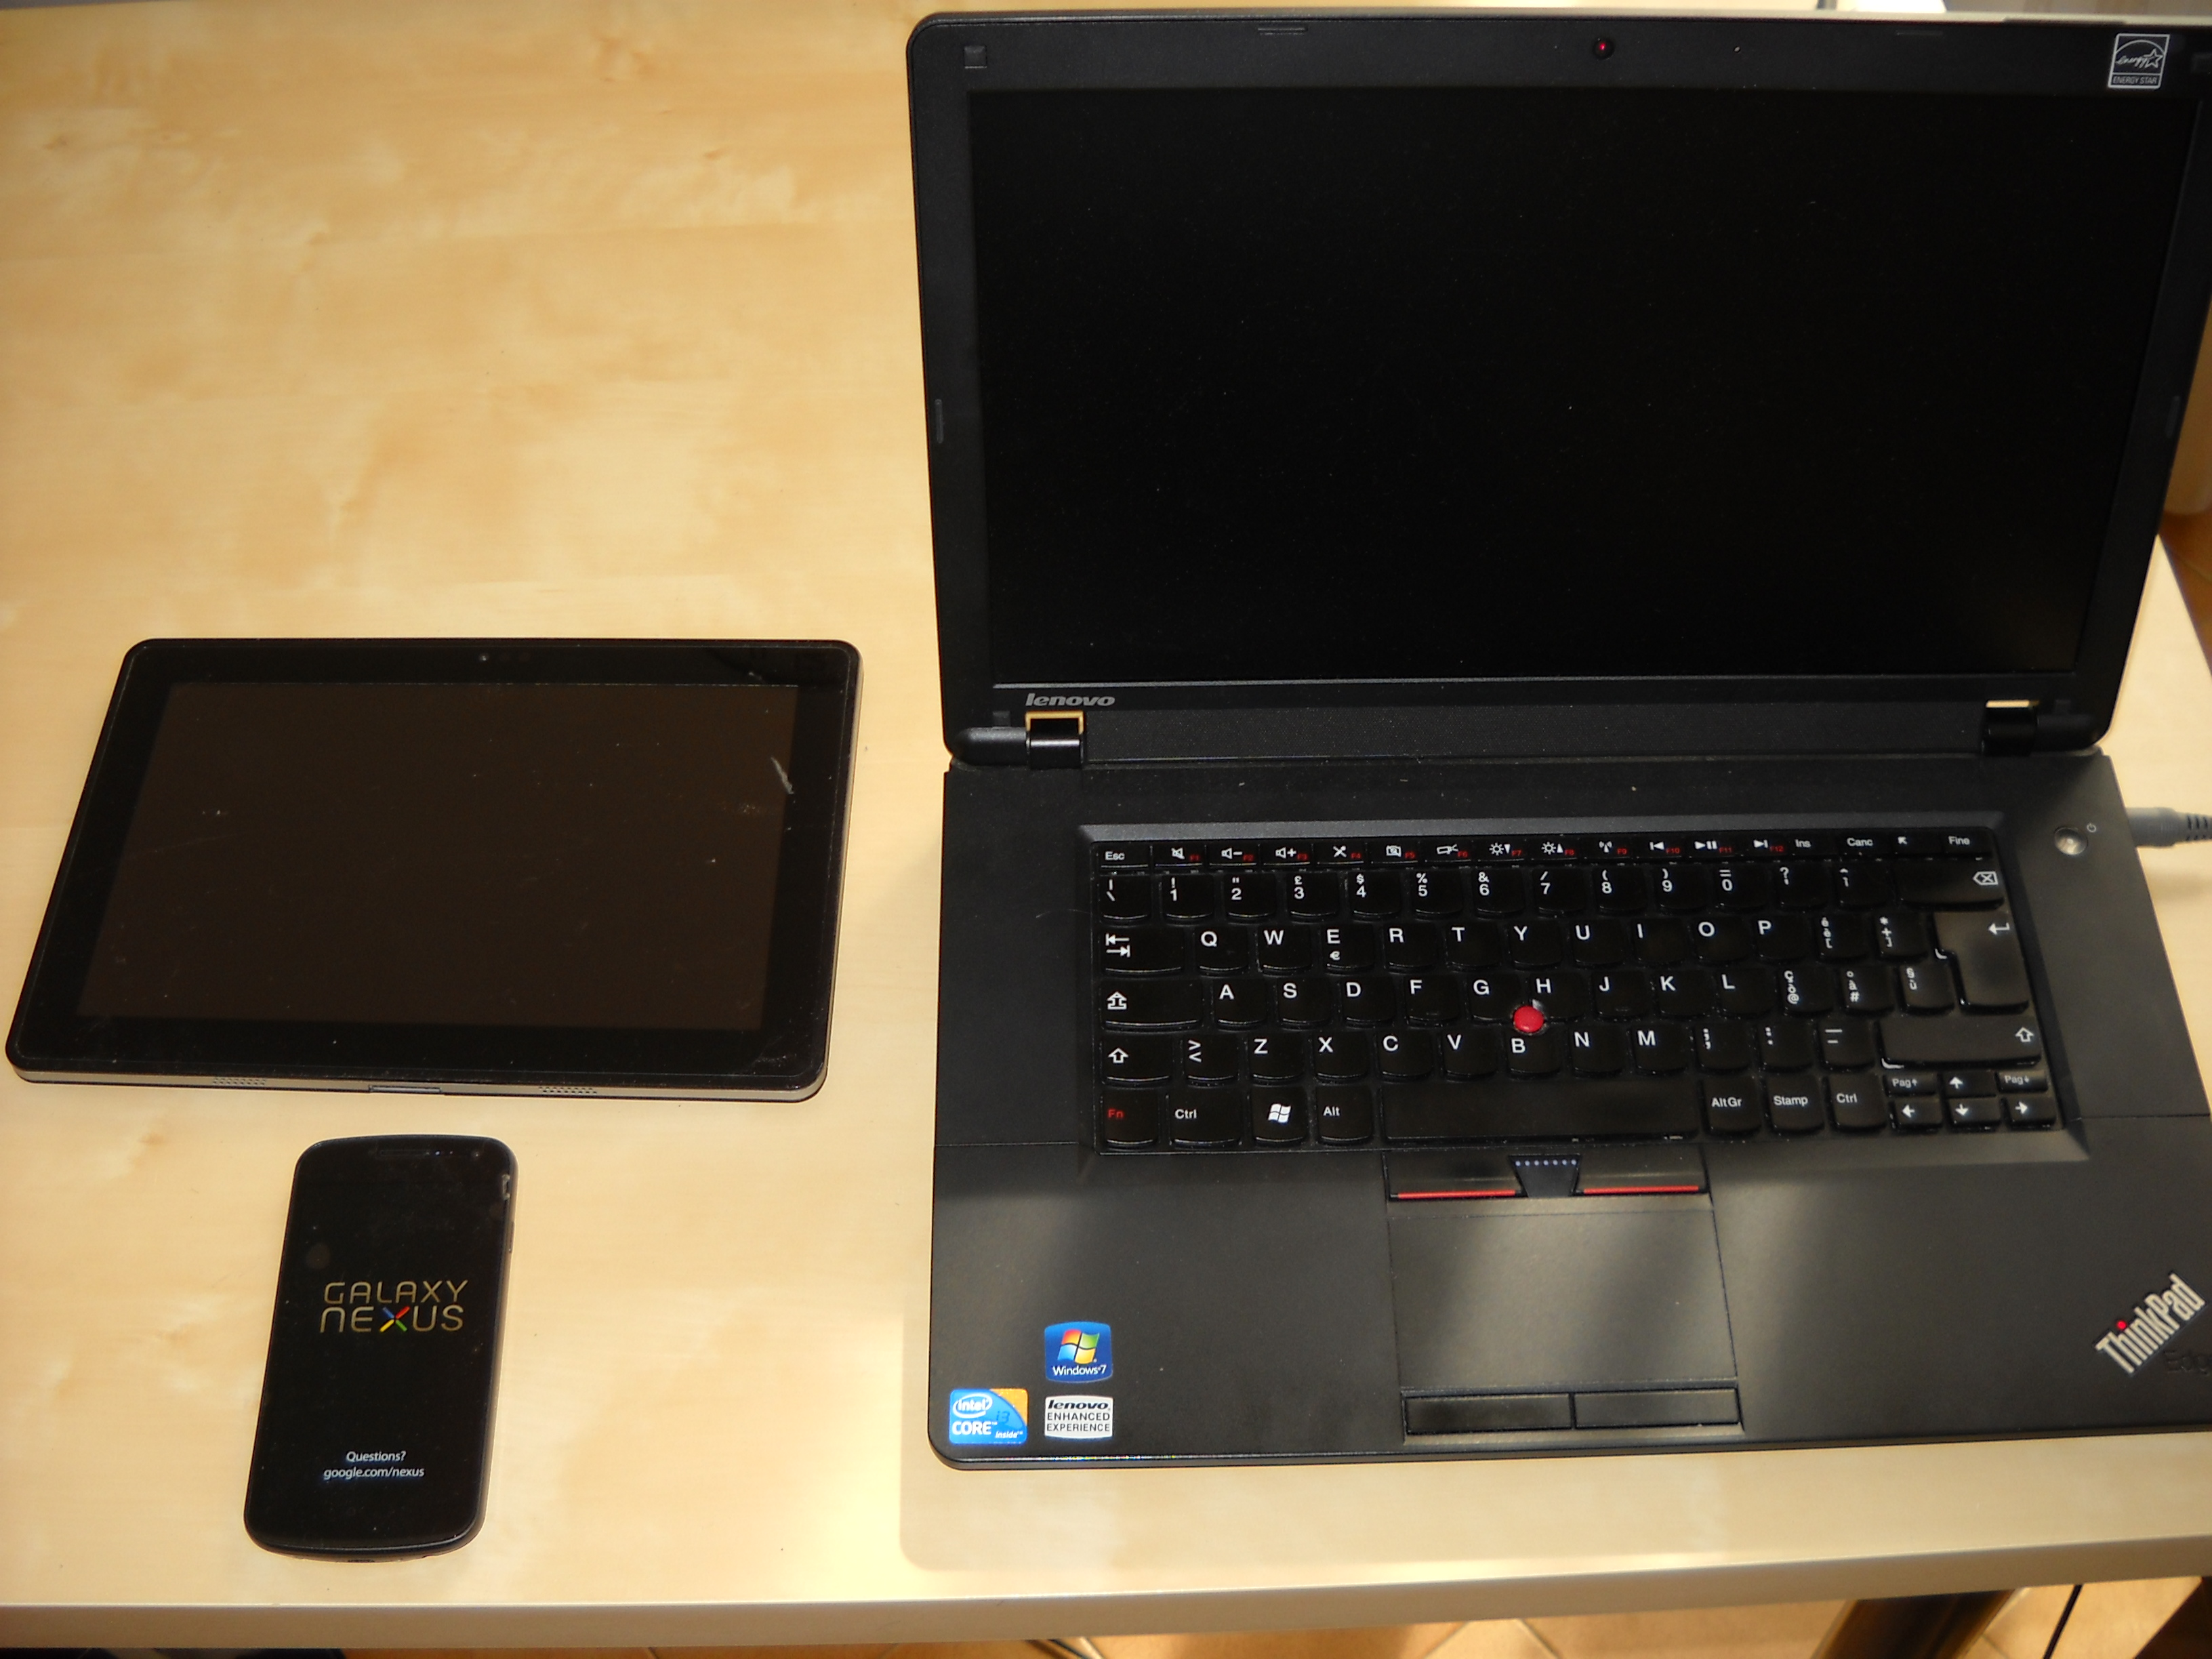
\includegraphics[scale=0.1]{img/lavoro.JPG}
\caption{\textit{Strumenti utilizzati per la realizzazione della tesi}.}
\label{fig:objofwork}
\end{figure}
